\chapter{Planificación y metodología}
\label{planificacion}

\section{Metodología utilizada}
\label{metodologia}
Aunque la realización de este proyecto no requiera en gran medida desarrollar un producto software complejo, 
se ha seguido la metodología de ''Issue Driven Development'' (IDD) con el fin de agilizar y organizar el trabajo.
Se trata de una metodología similar al ''Feature Driven Development'' en la cual la idea principal es que el 
estado actual y futuro del proyecto siempre quede reflejado en el sistema de tracking de issues que esté siendo utilizado.
Esta metodología presenta una serie de ventajas realmente interesantes como la modularidad que proporciona el que 
los commits y las ramas del repositorio sean autocontenidas, la granularidad gracias a que los commits y las ramas 
se centran exclusivamente en una issue actual a cerrar, además de poder llevar registro de las discusiones entre 
colaboradores con respecto a los commits realizados sobre una issue. Aunque esto último no nos atañe debido a que 
el proyecto está siendo desarrollado de forma individual, se trata de un punto positivo muy a tener en cuenta en 
entornos de desarrollo colaborativo.
El ''Issue Driven Development'' también se caracteriza por seguir una filosofía DRY o ''Don't Repeat Yourself'' en 
la que se incentiva el mantener de forma estructurada, unificada y centralizada toda la información de documentación 
con respecto a cambios y planificación de desarrollo con el fin de evitar problemas de redundancia y posible
fragmentación.\bigskip

El procedimiento a seguir en esta metodología empieza por la elección de un sistema de gestión de issues. Esto se 
comentará más adelante en ''\nameref{seguimiento}''. A continuación, antes de proceder con la realización de 
cualquier tarea, se crea una issue correspondiente en la quede reflejado qué se desea hacer y cómo se tiene planteado 
hacerlo. Es buena práctica agrupar issues por milestones para tener una visión más general de estas. Una vez 
creadas la issue en cuestión y su milestone correspondiente, se creará una rama en la que se llevará a cabo todo el 
desarrollo relacionado con la issue. Los commits que se realicen a las ramas deberán de contener una descripción 
explicativa de los cambios e incluir en el título una categoría y una referencia a la issue que se está tratando de solucionar. Con 
esto se busca que los commits tengan enlazada toda la información necesaria para comprender fácilmente los cambios 
realizados, es decir, que sean autocontenidos. Por último, una vez que la issue haya sido cerrada a través de un 
commit, se realizará un merge de la rama temática con la rama master.

Como es posible imaginar, esta metodología puede llegar a ser un tanto abrumadora en proyectos pequeños o poco 
complejos en los cuales puede darse el caso de que el esfuerzo de documentar en el sistema de gestión de issues 
todas las tareas a realizar puede llevar más tiempo que la realización de las tareas en sí.

Por último, comentar que para la toma de apuntes sobre la información de interés encontrada y y el desarrollo de 
las pruebas de concepto, se ha utilizado la herramienta de Joplin, una herramienta Open Source multiplataforma que 
permite tomar notas de manera organizada en formato Markdown. El poder mantener un formato constante para los apuntes
realizados en Joplin y los readme del repositorio de trabajo ha sido de gran ayuda para facilitar su traslado.

\section{Temporización}
Para realizar una estimación de la duración en días y el número de horas que pueden ocupar las distintas tareas que se desea 
llevar a cabo, se hace uso de un diagrama de Gantt en el cual quede reflejada toda esta información. Un diagrama de 
Gantt es una herramienta que tiene como objetivo ayudar en la gestión de proyectos. Suele estar compuesto por una lista 
de tareas a la izquierda y un cronograma de barras a la derecha para representar de forma visual la extensión de dichas 
tareas en el tiempo. Haciendo uso de la aplicación web \hyperlink{https://www.teamgantt.com/}{TeamGantt}, se crea el 
diagrama de la figura \ref{fig:gantt}.\bigskip
\begin{figure}
    \centering{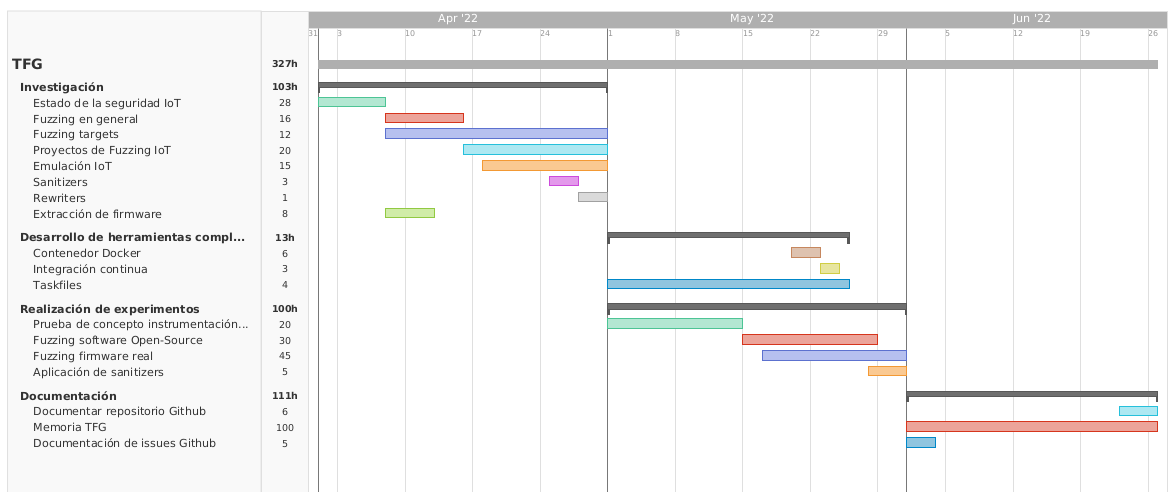
\includegraphics[scale=0.3]{Gantt.png}}
    \caption{Diagrama de Gantt con la planificación preliminar del proyecto.}
    \label{fig:gantt}
\end{figure}

La realización del proyecto se reparte en tres meses durante los cuales se plantean una serie de tareas generales a completar,
agrupadas en cuatro categorías principales, ''Investigación'', ''Desarrollo de herramientas complementarias'', ''Realización de 
experimentos'' y ''Documentación''. El siguiente listado de tareas queda reflejado en \ref{fig:gantt}:
\begin{itemize}
    \item \textbf{Investigación}: 
    \begin{itemize}
        \item \textbf{Estado de la seguridad IoT}: Como primera tarea del proyecto se ha de investigar la situación actual de la seguridad
        en el campo del internet de las cosas para tener un punto de partida.
        \item \textbf{Fuzzing en general}: Es necesario investigar el funcionamiento de la técnica del fuzzing en sí antes de proceder a 
        investigar sobre su aplicación al campo del IoT.
        \item \textbf{Fuzzing targets}: Se investigarán distintos dispositivos y sus respectivos firmware para descubrir software de interés
        sobre el que realizar fuzzing.
        \item \textbf{Proyectos de fuzzing IoT}: Como parte del estudio del estado del arte se investigarán las distintas técnicas y herramientas 
        aplicadas actualmente en la materia.
        \item \textbf{Emulación IoT}: Dado que la emulación es un factor clave en el fuzzing IoT será necesario profundizar en las distintas 
        técnicas disponibles.
        \item \textbf{Sanitizers}: Los sanitizers suelen ser utilizados para agilizar el proceso de fuzzing. Debemos de investigar cómo difiere
        su aplicación en dispositivos IoT con respecto a su uso tradicional.
        \item \textbf{Rewriters}: Investigar sobre esta nueva técnica que puede aumentar la eficiencia del fuzzing.
        \item \textbf{Extracción de firmware}: Como paso previo a aplicar fuzzing es necesario obtener los binarios que serán objeto de
        experimento. Investigaremos la metodología actual para extraer binarios a partir de una imagen firmware.
    \end{itemize}
    \item \textbf{Desarrollo de herramientas complementarias}:
    \begin{itemize}
        \item \textbf{Contenedor Docker}: Querremos desarrollar un contenedor Docker que evite tener que lidiar con la gran cantidad de dependencias 
        y paquetes software necesarios para realizar fuzzing orientado a IoT.
        \item \textbf{Integración continua}: Aplicando los conocimientos obtenidos en la asignatura de ''Infraestructura Virtual'' del grado de
        ingeniería informática de la UGR, se automatizará la publicación del contenedor Docker a DockerHub mediante CI/CD.
        \item \textbf{Taskfiles}: Aplicando también los conocimientos obtenidos en la asignatura de IV, se hará uso de un taskrunner que 
        facilitará la reproducibilidad de los experimentos. 
    \end{itemize}
    \item \textbf{Realización de experimentos}:
    \begin{itemize}
        \item \textbf{Prueba de concepto instrumentación dinámica}: Como introducción al fuzzing IoT, crearemos una prueba de concepto sobre
        un binario simple que nos permita familiarizarnos con las herramientas utilizadas y conocer las capacidades de la instrumentación dinámica.
        \item \textbf{Fuzzing software Open-Source}: Una vez se ha ganado algo de soltura con las herramientas a utilizar, se aplicará fuzzing 
        sobre un proyecto de código abierto orientado a sistemas empotrados.
        \item \textbf{Fuzzing firmware real}: Se llevará a cabo un experimento donde se aplique fuzzing a binarios extraídos del firmware de un 
        dispositivo real con el fin de identificar una vulnerabilidad conocida. 
        \item \textbf{Aplicación de sanitizers}: Para finalizar, se hará uso de sanitizers en los distintos ejemplos para analizar de qué forma 
        su uso influye en el proceso de fuzzing.
    \end{itemize}
    \item \textbf{documentación}:
    \begin{itemize}
        \item \textbf{Documentar repositorio Github}: El repositorio donde llevar a cabo el control de cambios del proyecto será 
        adecuadamente documentado a través de la redacción de diversos READMEs para sus distintas secciones.
        \item \textbf{Documentación de issues Github}: Dado que van a usarse diversas herramientas de código abierto activamente 
        desarrolladas a día de hoy, será necesario documentar a través de issues en los repositorios de proyecto correspondientes
        los distintos bugs que se encuentren en estos durante la realización de los experimentos.
        \item \textbf{Memoria TFG}: Todo el desarrollo del proyecto de principio a fin deberá de quedar reflejado en una memoria final.
    \end{itemize}
\end{itemize}

\section{Seguimiento del desarrollo}
\label{seguimiento}
Github ha sido la plataforma de control de cambios elegida debido a que junto con Git, han sido ampliamente utilizados
en las distintas asignaturas del grado de Ingeniería Informática y ya se parte conociendo su funcionamiento y dinámica de 
trabajo. Github proporciona una funcionalidad de tablero Kanban (Figura \ref{fig:kanban}) que combinado con lo comentado en ''\nameref{metodologia}''
nos permite de un vistazo ver el estado actual de las tareas del proyecto mediante su clasificación en una serie de columnas 
definidas que agrupan las issues según si se tratan de issues por comenzar, issues en progreso, issues bloqueadas a espera 
de arreglos en software de terceros o issues completadas. Podemos observar un ejemplo de issue creada durante la realización de los 
experimentos planteados en la figura \ref{fig:issue}.
\begin{figure}
    \centering{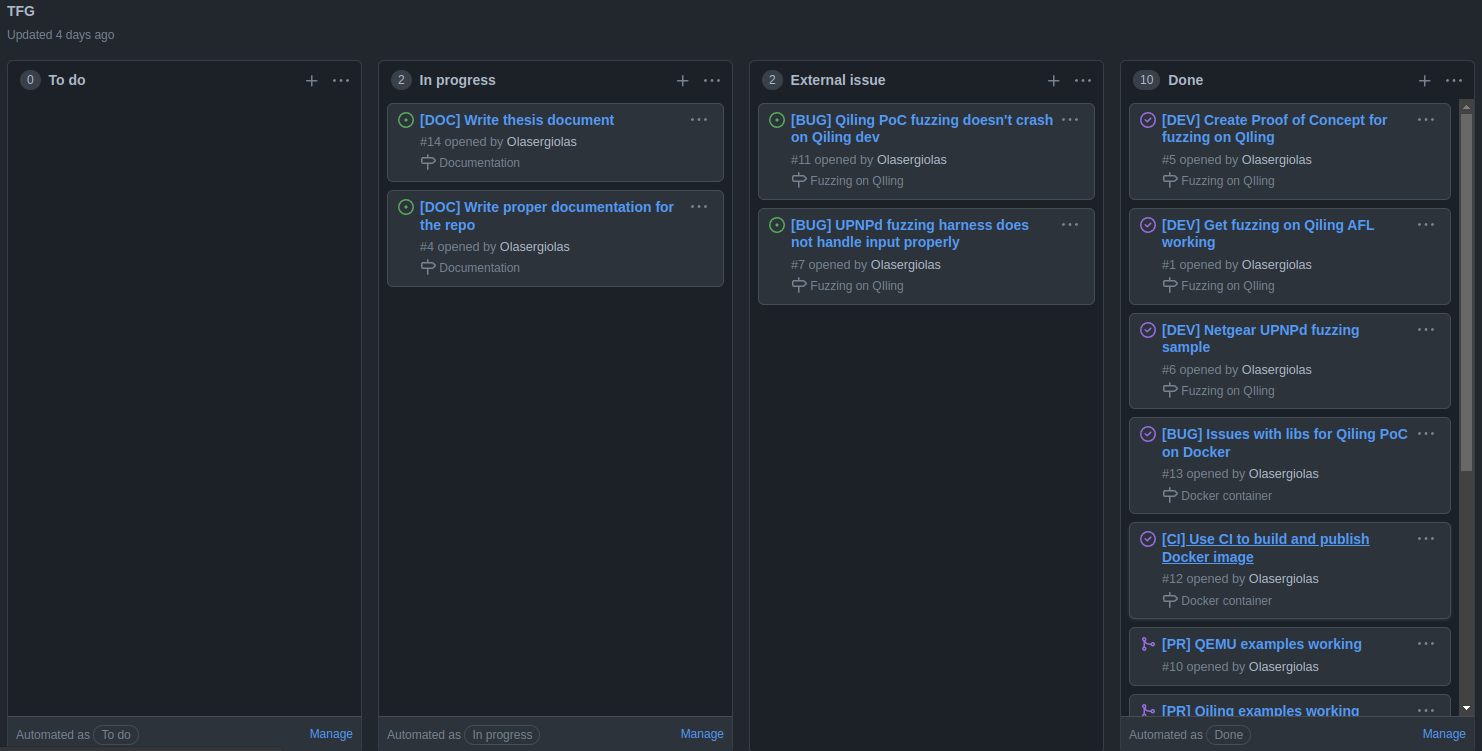
\includegraphics[scale=0.24]{kanban.png}}
    \caption{Funcionalidad de tablero Kanban de Github.}
    \label{fig:kanban}
\end{figure}

\begin{figure}
    \centering{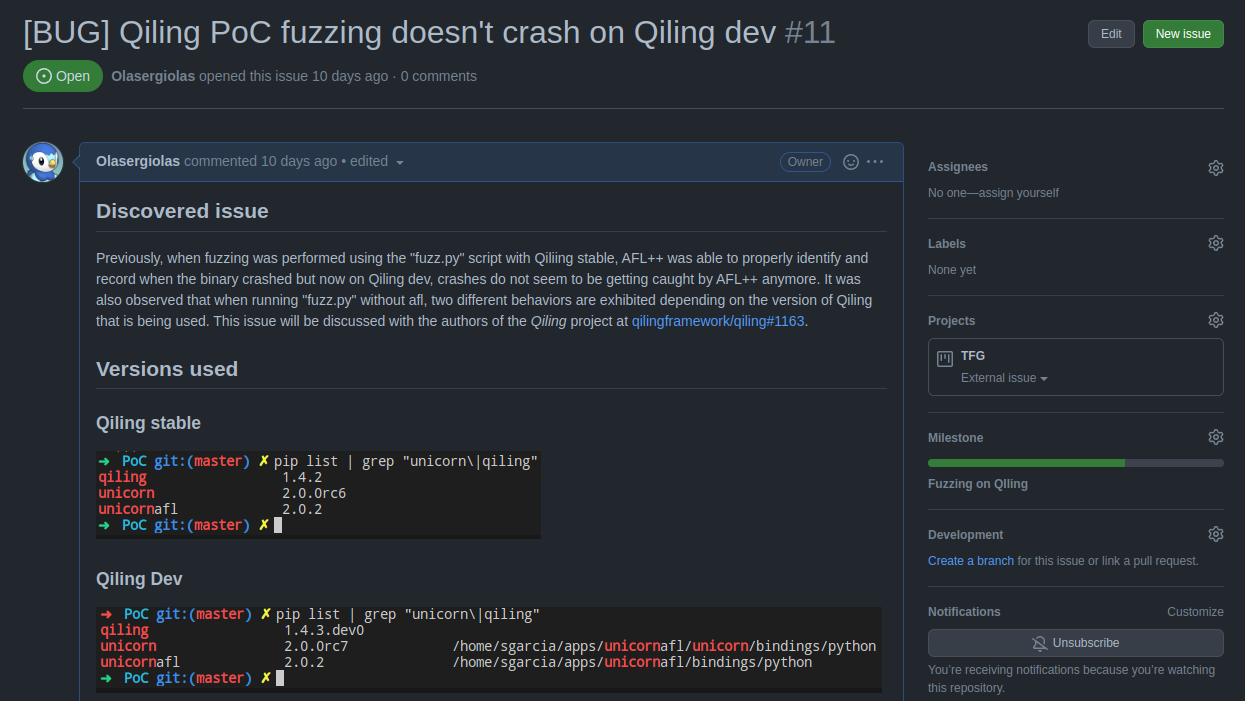
\includegraphics[scale=0.28]{issue.png}}
    \caption{Ejemplo de \href{https://github.com/Olasergiolas/TFG/issues/11}{issue} de reporte de bug en el repositorio del proyecto.}
    \label{fig:issue}
\end{figure}